\subsection{Propriedades Matemáticas}

% Organizar em subsubsections???
% primos, mod, probabilidade, combinatória

\begin{small}

% \subsubsection{Etc}
\begin{itemize}

    \item \textbf{Lagrange:} Todo número inteiro pode ser representado como soma de 4 quadrados.

    \item \textbf{Zeckendorf:} Todo número pode ser representado como soma de números de Fibonacci diferentes e não consecutivos.

    \item \textbf{Tripla de Pitágoras (Euclides):} Toda tripla pitagórica primitiva pode ser gerada por $(n^2 - m^2, 2nm, n^2 + m^2)$ onde $n$ e $m$ são coprimos e um deles é par.
    
    \item \textbf{Progressão Geométrica:} $S_n = a_1 \cdot \frac{q^n - 1}{q - 1}$

    \item \textbf{Soma dos Cubos:} $\sum_{k=1}^{n} k^3 = \left( \sum_{k=1}^{n} k \right)^2$
    
    \item \textbf{Chicken McNugget:} Para dois coprimos $x$ e $y$, o número de inteiros que não podem ser expressos como $ax + by$ é $(x-1)(y-1)/2$. O maior inteiro não representável é $xy - x - y$.

    \item\textbf{Primos até 200:} 2, 3, 5, 7, 11, 13, 17, 19, 23, 29, 31, 37, 41, 43, 47, 53, 59, 61, 67, 71, 73, 79, 83, 89, 97, 101, 103, 107, 109, 113, 127, 131, 137, 139, 149, 151, 157, 163, 167, 173, 179, 181, 191, 193, 197, 199

    \item\textbf{Fibonacci} $[0,20]$: 
    0, 1, 1, 2, 3, 5, 8, 13, 21, 34, 55, 89, 144, 233, 377, 610, 987, 1597, 2584, 4181, 6765.
    
    \item\textbf{Fatorial} $[0,15]$:
    1, 1, 2, 6, 24, 120, 720, 5040, 40320, 362880, 3628800, 39916800, 479001600, 6227020800, 87178291200, 1307674368000.
    
    \item\textbf{Potencias}
    \\
    \textbf{$2^n$} $[1,16]$: 
    2, 4, 8, 16, 32, 64, 128, 256, 512, 1024, 2048, 4096, 8192, 16384, 32768, 65536
    \\
    \textbf{$3^n$} $[1,13]$: 3, 9, 27, 81, 243, 729, 2187, 6561, 19683, 59049, 177147, 531441, 1594323
    \\
    \textbf{$5^n$} $[1,12]$: 
    $5$, $25$, $125$, $625$, $3125$, $15625$, $78125$, $390625$, $1953125$, $9765625$, $48828125$, $244140625$
    \\
    \textbf{$7^n$} $[1,9]$: 
    7, 49, 343, 2401, 16807, 117649, 823543, 5764801, 40353607, 282475249

    \item\textbf{Totiente de Euler:} $\varphi(n)$ conta quantos números entre 1 e $n$ são coprimos com $n$. \\
    Seq.$[1,32]$: 1, 1, 2, 2, 4, 2, 6, 4, 6, 4, 10, 4, 12, 6, 8, 8, 16, 6, 18, 8, 12, 10, 22, 8, 20, 12, 18, 12, 28, 8, 30
    
\end{itemize}
\subsubsection*{Primos}
\begin{itemize}
    \item\textbf{Goldbach:} Todo número par $n > 2$ pode ser representado como $n = a + b$, onde $a$ e $b$ são primos.

    \item\textbf{Primos Gêmeos:} Existem infinitos pares de primos $p$, $p + 2$.

    \item\textbf{Legendre:} Sempre existe um primo entre $n^2$ e $(n+1)^2$.

    \item\textbf{Wilson:} $n$ é primo se e somente se $(n-1)! \mod n = n - 1$.

\end{itemize}
\subsubsection*{Combinatória}
\begin{itemize}

    \item \textbf{Propriedades de Coeficientes Binomiais:}
    % \begin{align*}
    % \end{align*}
    % \vspace{-2pt}

    \begin{alignat*}{3}
        &\binom{n}{k} = \binom{n}{n - k} = \frac{n}{k} \binom{n - 1}{k - 1}, \\
        &\sum_{i=0}^{k} \binom{m}{i} \binom{n}{k-i} = \binom{m+n}{k},
        &\sum_{i=0}^{m} \binom{n}{i} (-1)^i = \binom{n - 1}{m}  (-1)^m       \\
        &\sum_{i=0}^{n} \binom{n}{i} = 2^n                         , \quad      
        &\sum_{i=0}^{n} \binom{n}{i} i = n \cdot 2^{n - 1}         , \qquad\qquad\quad
        &\sum_{i=0}^{n} \binom{i}{k} = \binom{n+1}{k+1}            ,           \\
        &\sum_{i=0}^{n} \binom{n-i}{i} = F_{n+1}                   ,
        &\sum_{i=0}^{m} \binom{n + i}{i} = \binom{n + m + 1}{m}    ,   \quad
        &\sum_{i=0}^{n} \binom{n}{i}^2 = \binom{2n}{n}                        \\
    \end{alignat*}


    \item\textbf{Triângulo de Pascal} \\[0.5ex]
    \begin{center} 
        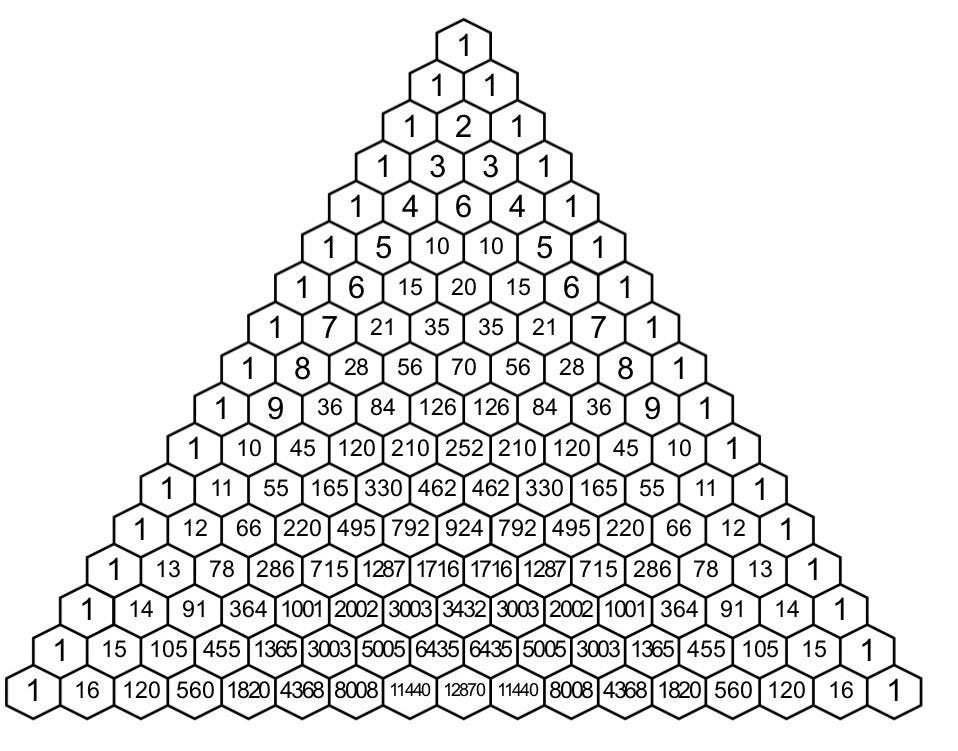
\includegraphics[width=0.75\linewidth]{math/pascal} 
    \end{center}
    
    \item\textbf{Números de Catalan:} expressões de parênteses bem formadas, \#binary trees com n+1 nodes, etc. $C_0 = 1$, e:
    \[ C_n = \frac{1}{n+1} \binom{2n}{n} = \sum_{i=0}^{n-1} C_i C_{n-1-i} \]
    Seq.$[0, 20]$: 1, 1, 2, 5, 14, 42, 132, 429, 1430, 4862, 16796, 58786, 208012, 742900, 2674440, 9694845, 35357670, 129644790, 477638700, 1767263190, 6564120420.

    \item\textbf{Burnside Lemma:} Número de colares diferentes (sem contar rotações), com $m$ cores e comprimento $n$:
    \[ \frac{1}{n} \left(m^n + \sum_{i=1}^{n-1} m^{\gcd(i, n)} \right) \]
    
    \item \textbf{Inversão de Möbius:} Útil para inclusão e exclusão nos primos. Seq.$[1, 30]$: 1, -1, -1, 0, -1, 1, -1, 0, 0, 1, -1, 0, 1, 1, 0, -1, 1, 0, 0, 1, -1, 1, 0, -1, -1, 0, 1, 0, 0, 1.
    $ \sum_{d \mid n} \mu(d) = 0 \ \ \text{if} \ \ n > 1 \ \text{else} \ 1 $ 


\item\textbf{Lindström-Gessel-Viennot:} A quantidade de caminhos disjuntos em um grid pode ser computada como o determinante da matriz do número de caminhos.


    \item \textbf{Numeros de Stirling:}
    \begin{itemize}
        \item \textbf{First Type:} 
         $|s(n,m)|$ é definido como a quantidade de permutações de $n$ elementos que contém exatamente $m$ ciclos de permutação. Tem aplicações em inclusão e exclusão.
        
        \[
        \left[{n \atop k}\right]  \quad=\quad 
        (n-1) \left[{ n-1 \atop k }\right] + \left[{n-1 \atop k-1}\right] 
        \quad=\quad (-1)^{n-k}s(n,k)
        \]
        \[
        \left[{n \atop 1}\right] = (n-1)! \quad , \quad
        \left[{n \atop n}\right] = 1 \quad , \quad
        \left[{n+1 \atop m+1}\right] = \sum_{i} \left[{n \atop i}\right] \binom{i}{m}
        \]
        
        \[\begin{array}{r||rrrrrrr}
        n|k & 0 & 1 & 2 & 3 & 4 & 5 & 6   \\\midrule
        0 & 1 &      &     &     &     &     &   \\
        1 &   & 1    &     &     &     &     &   \\
        2 &   & -1   & 1   &     &     &     &   \\
        3 &   & 2    & -3  & 1   &     &     &   \\
        4 &   & -6   & 11  & -6  & 1   &     &   \\
        5 &   & 24   & -50 & 35  & -10 & 1   &   \\
        6 &   & -120 & 274 & -225& 85  & -15 & 1 \\
        \end{array}\]
        
        
        \item \textbf{Second Type:} O Stirling set 
        ${\left\{{n \atop k}\right\}}$ conta maneiras de  particionar um conjunto de $n$ elementos em $k$ sub-conjuntos não vazios. 
        Equivalente a Rhyming Schemes de $n$ posições e $k$ símbolos. (exemplo n=3: k=1 \{aaa\}; k=2 \{aab, aba, abb\}; k=3 \{abc\})
        
        \[
        \left\{{n \atop k}\right\}  =
        k \left\{{n-1 \atop k}\right\} + \left\{{n-1 \atop k-1}\right\}
        \]
        \[
        \left\{{n \atop 1}\right\} = \left\{{n \atop n}\right\} = 1 \quad , \quad
        \left\{{n+1 \atop k+1}\right\} = \sum_{i} \left\{{i \atop k}\right\} \binom{n}{i}
        \]
        
        \[\begin{array}{r||rrrrrrr}
        n|k & 0 & 1 & 2 & 3 & 4 & 5 & 6 \\\midrule
        0 & 1 &   &   &   &   &   &     \\
        1 &   & 1 &   &   &   &   &     \\
        2 &   & 1 & 1 &   &   &   &     \\
        3 &   & 1 & 3 & 1 &   &   &     \\
        4 &   & 1 & 7 & 6 & 1 &   &     \\
        5 &   & 1 & 15 & 25 & 10 & 1 &   \\
        6 &   & 1 & 31 & 90 & 65 & 15 & 1 \\
        \end{array}\]

    \end{itemize}

    \item \textbf{Números de Bell $B_n$:} numero de partições de um conjunto de $n$ elementos. $ B_n =  \sum_{i} \left\{{n \atop i}\right\}  = \sum_{i} \binom{n-1} {i} B_i $. 
$[0,12]$: 1, 1, 2, 5, 15, 52, 203, 877, 4140, 21147, 115975, 678570, 4213597.


\item \textbf{Eulerian numbers (first order):}

O Eulerian number $\left\langle{n\atop k}\right\rangle$ ou $A(n,k)$ conta o número de permutações de tamanho $n$ com exatamente $k$ \emph{ascents} ($p_i<p_{i+1}$).

\[ 
\left\langle{n\atop k}\right\rangle 
\ = \ \ 
(k+1) \left\langle{n-1\atop k}\right\rangle  +  (n-k)\left\langle{n-1\atop k-1}\right\rangle 
\ \ \ =\ \ 
\sum_{i=0}^{k} (-1)^i \binom{n+1}{i}\,(k+1-i)^n
\]

\[
\left\langle{1\atop 0}\right\rangle = 1 
, \qquad 
\left\langle{n \atop 1}\right\rangle = 2^n - n - 1 
, \qquad 
\sum_{k=0}^{n-1} \left\langle{n\atop k}\right\rangle = n!
 \]


\[
\begin{array}{r|rrrrrrr}
n|k & 0 & 1 & 2 & 3 & 4 & 5 & 6\\\midrule
1 & 1 & & & & & & \\
2 & 1 & 1 & & & & & \\
3 & 1 & 4 & 1 & & & & \\
4 & 1 & 11 & 11 & 1 & & & \\
5 & 1 & 26 & 66 & 26 & 1 & & \\
6 & 1 & 57 & 302 & 302 & 57 & 1 & \\
7 & 1 & 120 & 1191 & 2416 & 1191 & 120 & 1\\
\end{array}
\]


\end{itemize}
\subsubsection*{Modular}
\begin{itemize}

    \item \textbf{Fermat:} Se $p$ é primo, então $a^{p-1} \equiv 1 \mod p$. Se $x$ e $m$ são coprimos e $m$ primo, então $x^k \equiv x^{k \bmod (m-1)} \mod m$.
          \textit{Euler:} $x^{\varphi(m)} \equiv 1 \mod m$. $\varphi(m)$ é o totiente de Euler.


    \item \textbf{Teorema Chinês do Resto:} Dado um sistema de congruências:
    $ x \equiv a_1 \mod m_1, \quad \ldots, \quad x \equiv a_n \mod m_n $
    com $m_i$ coprimos dois a dois. E seja $M_i = \frac{m_1 m_2 \cdots m_n}{m_i}$ e $N_i = M_i^{-1} \mod m_i$. Então a solução é dada por $x = \sum_{i=1}^{n} a_i M_i N_i $
    Outras soluções são obtidas somando $m_1 m_2 \cdots m_n$.

\end{itemize}
\subsubsection*{Probabilidade}
\begin{itemize}

    \item \textbf{Bertrand Ballot:} Com $p > q$ votos, a probabilidade de sempre haver mais votos do tipo $A$ do que $B$ até o fim é:
    $ \frac{p - q}{p + q} $
    Permitindo empates: 
    $\frac{p + 1 - q}{p + 1}$. Multiplicando pela combinação total $\binom{p + q}{q}$, obtém-se o número de possibilidades.

    
    \item \textbf{Linearidade da Esperança:} $E[aX + bY] = aE[X] + bE[Y]$

    \item \textbf{Variância:} $\text{Var}(X) = E[(X - \mu)^2] = E[X^2] - E[X]^2$

    \item \textbf{Uniforme:} $X \in \{a, a+1, \dots, b\}$, $E[X] = \frac{a + b}{2}$
        
    \item \textbf{Binomial:} $n$ tentativas com probabilidade $p$ de sucesso:
    $ P(X = x) = \binom{n}{x} p^x (1 - p)^{n - x}, \quad E[X] = np $
    
    \item \textbf{Geométrica:} Número de tentativas até o primeiro sucesso:
    $ P(X = x) = (1 - p)^{x - 1} p, \quad E[X] = \frac{1}{p} $

\end{itemize}
\end{small}
% credits: https://github.com/gabrielpessoa1/ICPC-Library/